

\documentclass{beamer}
\usepackage{graphicx}
\usepackage{bm}
\title{}
\subtitle{Hierarchical models for estimating state and
	demographic trends in US death penalty public
	opinion}


\date{\today}

\begin{document}
	\begin{frame}
		\maketitle
	\end{frame}
	
	\begin{frame}{Goal}
		\begin{itemize}
			\item Goal of this paper is to understand the trends of public opinion on the death penalty
			\item Mainly descriptive analysis, no attempt at causation parameter
			\item Try to predict support probability by demographic information
			\item Use information that can be gathered about location as explanatory variable
		\end{itemize}
	\end{frame}
	
	\begin{frame}{How to accomplish goals}
		\begin{itemize}
			\item Data used in the paper
		\end{itemize}
		\begin{figure}
			\centering 
			\includegraphics[scale=.4]{fwf}
		\end{figure}
	\end{frame}
	
	\begin{frame}{Descriptive analysis match}
		From the authors paper:
		\begin{tabular}{cc}
				\includegraphics[scale=.2]{descriptive1} & 						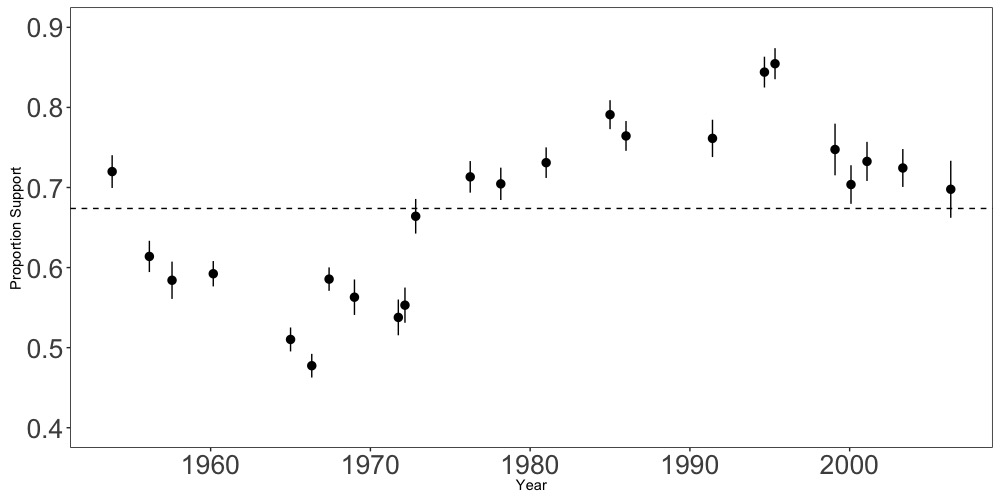
\includegraphics[scale=.15]{mydescriptive1} \\
		\end{tabular}
		\begin{figure}
			\centering

		\end{figure}
	\end{frame}
	
	\begin{frame}{Descriptive analysis match}
		\begin{tabular}{cc}
		\includegraphics[scale=.22]{descriptive2}&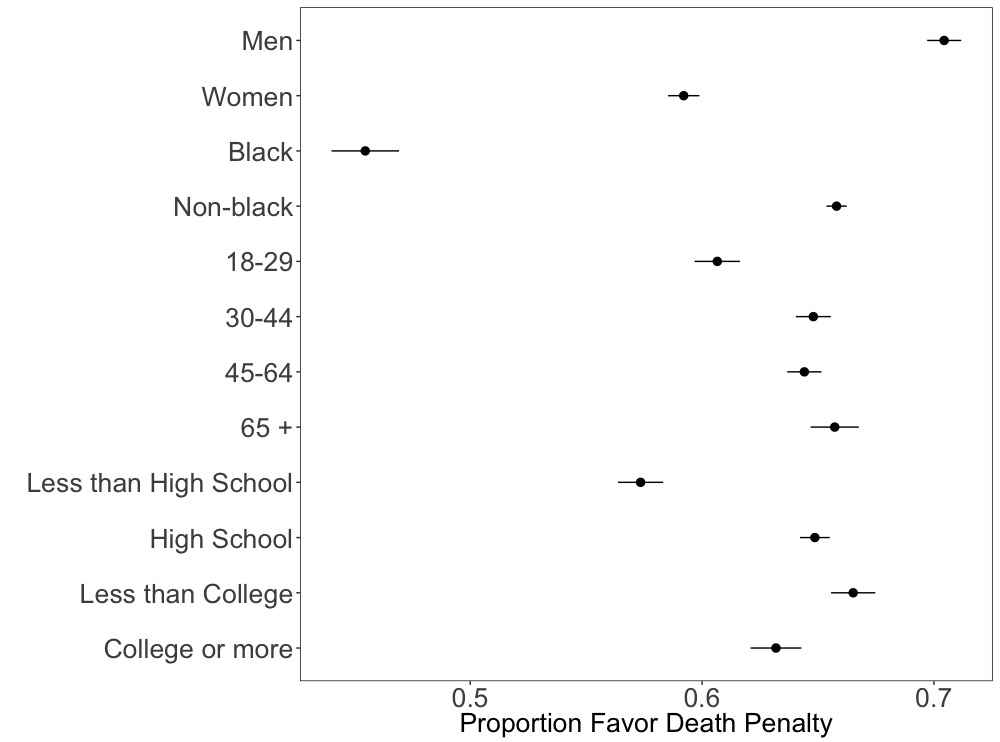
\includegraphics[scale=.15]{mydescriptive2} \\
		\end{tabular}
	\end{frame}
	
	\begin{frame}{Predicting support-Level 1}
		Use a logit model to predict support 
		\[ y_i = 1 \text{ in favor} \]
		\[  y_i = 0 \text{ o/w} \]
		\[ p(y_i = 1) = \frac{1}{1 + exp\{-\eta_i \}  } \]
	\end{frame}
	
	\begin{frame}{Factors in $ \eta_i $}

		\begin{itemize}
			\item The model contains thousands of parameters (8,466 in main model, not including variances and sub-level models!). 
			\item Not identified, use multiple levels to help identify parameters (Gelfand and Sahu, 1999)
		\end{itemize}
		\begin{description}
			\item[Factors in model] 
		\end{description}
			 $$ \eta_i = \alpha_{state_i, year_i} + \alpha_{degree_i, state_i} + \alpha_{age_i, state_i} +  $$
			 $$ \delta_{age_i, state_i}x^{(b)}_i + \beta_{black_i, state_i}x^{(b)}_ix^{(y)}_i  + $$
			 $$ \beta_{female_i, state_i} x^{(f)}_i +  \delta_{female_i, state_i}x^{(f)}_ix^{(y)}_i  + $$ 
		$$ \beta_{black_i, female_i, state_i}x^{(b)}_ix^{(f)}_i + \delta_{black_i, female_i, state_i}x^{(b)}_ix^{(f)}_ix^{(y)}_i $$
			\begin{itemize}
				\item Each parameter has its own model
			\end{itemize}
	\end{frame}

	\begin{frame}{Lower levels}
		The lower level models help identify parameters with few data points by `shrinking' towards regional and national averages
		Regression for state year interaction effect:
		\begin{equation}
		\alpha_{state_s,year_t} \sim N(\alpha_{year_t} + \alpha_{state_s} + \delta_{state_s}x_{year_t}, \sigma^2_{state, year})
		\end{equation}
		But each of these parameters has its own model!! \\ \begin{center} Time is a AR(1) \end{center}
		\begin{equation}
		\alpha_{year_t} \sim N(\mu + \mu_{\delta}x_{year_t} + \phi(\alpha_{year_t}  - \mu - \mu_{\delta} x_{year_{t-1}}), \sigma^2_{year})
		\end{equation}
		\begin{equation}
		\alpha_{year_1} \sim N(\mu + \mu_{\delta} x_{year_1}, \frac{\sigma^2_{year}}{(1-\phi^2)}  ) 
		\end{equation}
		Each of these has its own model!!!
	\end{frame}
	
	\begin{frame}{Lower levels of hell (hierarchy)}
		\begin{figure} 
			\centering
	\includegraphics[scale=.15]{dante}
	\caption{Dante in the 9th circle-replication match}
	\end{figure}
	\begin{itemize} 
		\item Think of $ \mu $ as a national average \textit{intercept term} $ \mu \sim N(0, 25)  $, weakly informative
		\item Think of $ \mu_{\delta} $ as a national average \textit{time trend} $ \mu_{\delta} \sim N(0, 25) $
	\end{itemize}
	\[
			\alpha_{year_1} \sim N\Big(\mu + \mu_{\delta} x_{year_1}, \frac{\sigma^2_{year}}{(1-\phi^2)}  \Big) 
	\]
	\end{frame}
	
	\begin{frame}{Lower levels of hierarchy - state interactions}
		\begin{figure}
				\includegraphics[scale=.12]{census_regions}
				\caption{Regions of U.S. according to U.S. Census}
		\end{figure}
		\begin{equation}
		\alpha_{state_s} \sim N(\alpha_{region_s} + \bm{\beta X}^{T}_{state_s}, \sigma^2_{region_s}   )
		\end{equation}
		$ \bm{\beta } = (\beta_1 \ \beta_2) $, $ \bm{X_}{state} = \begin{pmatrix}
		l_{1} & k_{1} \\
		l_{2} & k_{2} \\
		\vdots & \vdots \\
		l_{51} & k_{51} \\
		\end{pmatrix}$ legality $ l $, Republican share $ k $
	\end{frame}
	
	\begin{frame}{Even Lower levels}
		Republican Share...
		\begin{itemize}
			\item To get the values $ k_1, k_2, \dots, k_{50} $ I had to run 50 regressions! 
			\item And find the data for how each state voted...
									\item The regressions are \[ \text{Republican share} = k + \lambda t \] $ t $ a time vector 
									\item Each of these 50 regressions form the elements of $ \bm{X_}{state }$
		\end{itemize}
	\end{frame}
	
	\begin{frame}{Legality}
		\begin{itemize}
			\item Supreme Court decision \textit{Furman vs. Georgia}, 1972
			\item $ l_s $ is the percentage of time the death penalty was legal in the state during the sampling years, 1953-2006
			\item From the paper \begin{quotation}
				Iowa, West Virginia and the District of Columbia have never rewritten their death penalty statutes since 1972.
			\end{quotation}
			\item True, but some still had the death penalty \textit{before} these years
			\begin{quotation}
				10 states have never had a death penalty statute during this time span.
			\end{quotation}
			10 states? I find only 5. Mean and standard deviations come out to be 
			\begin{table}
				\begin{tabular}{lll}
					& Author & Replication \\
					\hline 
					\hline 
					$ \mu $& 0.70 & 0.75 \\
					sd & 0.39 & 0.33 \\
					\hline 
				\end{tabular}
			\end{table}
			
		\end{itemize}
	\end{frame}
	
	\begin{frame}{Lower levels of hierarchy}
		That is how one of the sub-hierarchies is obtained
			\[
			\alpha_{state_s} \sim N(\alpha_{region_s} + \bm{\beta X}^{T}_{state_s}, \sigma^2_{region_s}   )
			\]
			Ultimately we are after \dots
						 $$ \eta_i = \alpha_{state_i, year_i} + \alpha_{degree_i, state_i} + \alpha_{age_i, state_i} +  $$
						 $$ \delta_{age_i, state_i}x^{(b)}_i + \beta_{black_i, state_i}x^{(b)}_ix^{(y)}_i  + $$
						 $$ \beta_{female_i, state_i} x^{(f)}_i +  \delta_{female_i, state_i}x^{(f)}_ix^{(y)}_i  + $$ 
						 $$ \beta_{black_i, female_i, state_i}x^{(b)}_ix^{(f)}_i + \delta_{black_i, female_i, state_i}x^{(b)}_ix^{(f)}_ix^{(y)}_i $$
		\begin{itemize}
			\item Specify about 10,000 priors 
			\item Standard deviations, except for some exceptions are distributed $ t  \ \mathbb{I}_{1\in(0,+\infty)} $ $ \mu=0 $, scale =5, $ \nu =3 $ 
		\end{itemize}
		\end{frame}
	\begin{frame}{JAGS}
		Model run in JAGS for 10,000 iterations, 3 chains and thinned by 5. 
		\begin{itemize}
			\item Strategy to get predicted in sample fits
			\item There are so many parameters! Predicting $ p(y_i =1) $ for each data point would be very difficult
			\item Possible, and I did, obtain every posterior mean (all 8,000+)
			\item However, JAGS is able to monitor specific values
			\item Idea is to monitor the estimated probabilities $ \hat{\pi} $, 
			\[
			\hat{\pi} = \frac{1}{1 + \exp^{-\eta_i} }
			\]
			\item Compare with the mean of the observed values
		\end{itemize}
	\end{frame}
	
	\begin{frame}{Author's results}
		\begin{figure}
			\includegraphics[scale=.16]{results1}
		\end{figure}
		\begin{figure}
			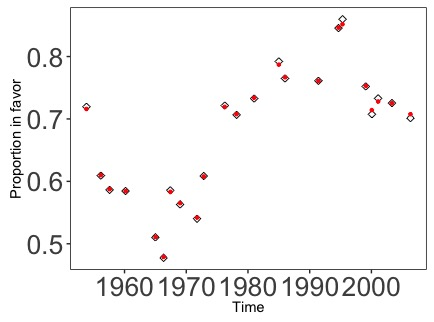
\includegraphics[scale=.3]{myresults}
			\caption{Actual vs. estimated in sample fit, Red Dots = In sample fits}
		\end{figure}
	\end{frame}
	
	\begin{frame}{In summary}
		\begin{itemize}
			\item I could not (because of time constraints) replicate \textbf{everything}
			\item However, so far I have replicated what I have attempted
			\item Fill in data for non-sampled years...take the coefficients corresponding to these years and multiply them by that part of the data
			\item 2,000 lines of code
		\end{itemize}
	\end{frame}
	
\end{document}